\section{Pianificazione delle attività}
\label{sez:pianificazione-attivita}

La pianificazione delle attività è stata effettuata seguendo un approccio iterativo e collaborativo, con l'obiettivo di garantire una gestione efficace del progetto.\\
Durante la prima settimana, ho lavorato alla definizione delle \gls{user-stories}, che hanno permesso di identificare e organizzare le funzionalità principali del progetto in base alla priorità e al valore per l’utente.\\
Per la lista delle \gls{user-stories} si veda la {\hyperref[subsubsec:epic-stories]{sezione §3.3.1}}.\\

\noindent Successivamente, insieme al \textit{tutor} aziendale, le attività sono state suddivise in \gls{sprint} settimanali.\\
In ogni \gls{sprint} abbiamo selezionato specifiche \gls{user-stories} da completare, tenendo conto delle loro priorità, mantenendo un carico di lavoro sostenibile per il periodo di una settimana. \\
Per ciascun \gls{sprint} sono stati definiti dei criteri di accettazione, ovvero parametri chiari e verificabili che indicano quando un'attività può essere considerata completata. \\
Questi criteri, stabiliti in collaborazione con il \textit{tutor} aziendale, hanno assicurato una qualità elevata del lavoro svolto ed una comprensione condivisa degli obiettivi. \\
Questo approccio ha permesso di monitorare costantemente i progressi e garantire un miglioramento continuo durante ogni iterazione del progetto.


\pagebreak
\subsection{Pianificazione settimanale}
\label{sez:pianificazione-settimanale}

\section*{\textit{Sprint} 1: Studio tecnologie (25 Settembre - 1 Ottobre)}
\textbf{Obiettivo:} Studio delle tecnologie fondamentali per il progetto, creazione \gls{user-stories} e della pianificazione.\\  

\noindent \textbf{Descrizione:}\\  
\noindent In questo \gls{sprint}, l'obiettivo principale è acquisire familiarità con le tecnologie che verranno utilizzate nel progetto, come \textit{AWS Bedrock}, \textit{AWS Cognito}, \textit{React}, \textit{NestJS}, \textit{MongoDB}, \textit{Puppeteer} ed altri strumenti correlati.\\
Ho inoltre stilato le \gls{user-stories} e la pianificazione settimanale.\\

\noindent \textbf{Criteri di accettazione:}  
\begin{itemize}
    \item Sono state create tutte le \gls{user-stories} necessarie per la pianificazione del progetto;
    \item È stata stilata una pianificazione dettagliata, suddivisa in \gls{sprint} settimanali, che definisce le attività principali del progetto;
    \item Lo stagista ha acquisito una conoscenza di base sufficiente delle tecnologie per iniziare le implementazioni nei successivi \gls{sprint}.
\end{itemize}
\section*{\textit{Sprint} 2: Implementazione autenticazione con \textit{AWS Cognito} (2 Ottobre - 8 Ottobre)}
\textbf{Obiettivo:} Implementare il sistema di autenticazione utilizzando \textit{AWS Cognito}.\\  

\noindent \textbf{Descrizione:}\\  
\noindent Questo \gls{sprint} si concentra sull'implementazione del flusso di \textit{login} per gli utenti utilizzando \textit{AWS Cognito}. \\
Ho sviluppato il sistema di autenticazione e autorizzazione, consentendo agli utenti di accedere e gestire il proprio \textit{account}. \\
Ho inoltre implementato messaggi di errore chiari in caso di credenziali errate.\\

\noindent \textbf{\textit{User Stories}:}  
\begin{itemize}
    \item \textbf{\textit{Login} nel sistema}: Come utente voglio poter accedere al sistema e visualizzare la \textit{dashboard} così da gestire i miei progetti precedenti e crearne di nuovi;
    \item \textbf{Errore di accesso in caso di credenziali errate}: Come utente, in caso di errore di accesso (es. \textit{password} errata), voglio essere informato con un messaggio chiaro su come risolvere il problema.
\end{itemize}

\noindent \textbf{Criteri di accettazione:}  
\begin{itemize}
    \item L'utente può accedere inserendo \textit{email} e \textit{password};
    \item Se le credenziali sono corrette, l'utente viene reindirizzato alla \textit{dashboard};
    \item Se le credenziali sono errate, l'utente vede un messaggio di errore con istruzioni per il recupero della \textit{password}.
\end{itemize}

\pagebreak
\section*{\textit{Sprint} 3: Visualizzazione, ricerca ed eliminazione dei progetti (9 Ottobre - 15 Ottobre)}
\noindent \textbf{Obiettivo:} Implementare la visualizzazione dei progetti e la loro ricerca.\\

\noindent \textbf{Descrizione:}\\  
\noindent In questo \gls{sprint}, ho sviluppato la funzionalità per visualizzare la lista dei progetti, cercare progetti specifici tramite l’applicazione di filtri e l’eliminazione di un progetto.\\  

\noindent \textbf{\textit{User Stories}:}  
\begin{itemize}
    \item \textbf{Visualizzazione lista progetti}: Come utente voglio poter vedere la lista di tutti i progetti precedentemente generati con annesso nome e data di creazione, così da poter scegliere quale selezionare;
    \item \textbf{Funzione ricerca e filtraggio progetti}: Come utente voglio poter cercare e filtrare i miei progetti per data o nome così da trovare facilmente il progetto desiderato anche in un elenco molto lungo;
    \item \textbf{Eliminazione di un progetto}: Come utente, voglio poter eliminare un progetto che ho creato in modo che possa rimuovere progetti non più necessari o irrilevanti.
\end{itemize}

\noindent \textbf{Criteri di accettazione:}  
\begin{itemize}
    \item L'utente può visualizzare una lista dei progetti con nome e data di creazione;
    \item L'utente può ricercare o filtrare un progetto per nome e/o data di creazione;
    \item L'utente può eliminare un progetto, con una finestra di conferma, e rimuovere definitivamente i dati.
\end{itemize}

\section*{\textit{Sprint} 4: Implementazione \textit{preset} e bozze di progetto (16 Ottobre - 22 Ottobre)}
\textbf{Obiettivo:} Implementare la pagina di creazione dei progetti, da cui è possibile compilare i \textit{preset} o salvarli come bozza.\\

\noindent \textbf{Descrizione:}\\
\noindent In questo \textit{sprint}, ho sviluppato la pagina per la compilazione dei \textit{preset}, da cui è inoltre possibile salvare una bozza compilata (in parte) per essere utilizzata in un secondo momento.\\
Ho inoltre sviluppato la pagina che contiene le informazioni di un singolo progetto, come nome, data di creazione e tutti i capitoli che lo compongono.\\  

\noindent \textbf{\textit{User Stories}:} 
\begin{itemize}
    \item \textbf{Visualizzazione singolo progetto}: Come utente voglio poter selezionare un singolo progetto salvato nella mia area personale così da visualizzarne i dettagli (nome, data di creazione, ecc.);
    \item \textbf{Visualizzazione descrizione \textit{preset}}: Come utente voglio visualizzare una descrizione dettagliata di ciascun \textit{preset} così da scegliere quello più adatto alle mie esigenze specifiche;
    \item \textbf{Salvataggio \textit{preset} compilato}: Come utente voglio poter salvare il \textit{preset} compilato così da poterlo completare e generare il documento in un momento successivo.
\end{itemize}

\noindent \textbf{Criteri di accettazione:}  
\begin{itemize}
    \item L’utente può visualizzare le informazioni di un progetto dalla sua pagina di visualizzazione;
    \item L'utente può selezionare un \textit{preset} dalla lista e leggerne la descrizione ed i casi d’uso per cui può essere utilizzato;
    \item L'utente può salvare un \textit{preset} compilato parzialmente per completarlo in seguito.
\end{itemize}

\section*{\textit{Sprint} 5: Generazione progetti e \textit{download} PDF (23 Ottobre - 29 Ottobre)}
\textbf{Obiettivo:} Implementare la generazione di progetti ed il \textit{download} dei documenti in formato PDF.\\

\noindent \textbf{Descrizione:}\\
\noindent Questo \textit{sprint} si concentra sulla generazione dei progetti utilizzando i \textit{preset} e sulla possibilità di scaricare il progetto finale in formato PDF.\\
L'utente può scaricare il documento completo per l'archiviazione e/o la condivisione.\\

\noindent \textbf{\textit{User Stories}:} 
\begin{itemize}
    \item \textbf{Generazione progetto tramite \textit{preset}}: Come utente voglio poter generare un progetto con l'aiuto di \textit{preset} predefiniti e ottimizzati, così da creare rapidamente un documento utile e strutturato senza partire da zero;
    \item \textbf{\textit{Download} documento progetto}: Come utente voglio poter scaricare il progetto generato in formato PDF così da poterlo condividere facilmente con il mio \textit{team} o archiviare per un utilizzo futuro.
\end{itemize}

\noindent \textbf{Criteri di accettazione:}  
\begin{itemize}
    \item Il progetto può essere generato tramite \textit{preset}, utilizzando i servizi di \gls{generative-ai} offerti da \gls{aws};
    \item L'utente può scaricare il progetto generato come PDF;
    \item Il PDF contiene tutti i capitoli e le informazioni del progetto.
\end{itemize}

\pagebreak
\section*{\textit{Sprint} 6: Rigenerazione progetti e capitoli (30 Ottobre - 5 Novembre)}
\textbf{Obiettivo:} Implementare la rigenerazione dei progetti e la possibilità di rigenerare capitoli specifici.\\

\noindent \textbf{Descrizione:}\\
\noindent In questo \textit{sprint}, ho implementato la funzionalità per rigenerare un progetto completo o singoli capitoli, consentendo all'utente di modificare e aggiornare solo le parti necessarie del progetto, mantenendo intatti gli altri capitoli.\\

\noindent \textbf{\textit{User Stories}:} 
\begin{itemize}
    \item \textbf{Rigenerazione progetto}: Come utente voglio poter rigenerare un progetto, aggiungendo o modificando informazioni, così da ottenere diverse versioni del documento per meglio adattarsi alle mie esigenze;
    \item \textbf{Rigenerazione specifici capitoli}: Come utente voglio rigenerare specifici capitoli di un progetto già creato, mantenendo inalterati gli altri capitoli, così da aggiornare solo le sezioni che richiedono modifiche senza dover rigenerare tutto il documento.
\end{itemize}

\noindent \textbf{Criteri di accettazione:}  
\begin{itemize}
    \item L'utente può selezionare e rigenerare un progetto o specifici capitoli;
    \item La rigenerazione aggiorna solo le sezioni selezionate, mantenendo il resto del progetto invariato;
    \item La nuova versione rigenerata viene salvata come una nuova versione del progetto.
\end{itemize}

\section*{\textit{Sprint} 7: Gestione della versione e rifiniture finali (6 Novembre - 12 Novembre)}
\textbf{Obiettivo:} Gestire la versione dei progetti ed effettuare le rifiniture finali prima della fase di \textit{testing}.\\

\noindent \textbf{Descrizione:}\\
\noindent In questo \textit{sprint}, ho sviluppato la funzionalità per gestire la versione dei progetti, permettendo agli utenti di visualizzare, confrontare e ripristinare versioni precedenti.\\
Inoltre, ho completato le ultime rifiniture del sistema, inclusi eventuali miglioramenti all'interfaccia o risoluzioni di \textit{bug}.\\

\noindent \textbf{\textit{User Stories}:} 
\begin{itemize}
    \item \textbf{Visualizzazione versioni precedenti progetto}: Come utente voglio poter visualizzare le versioni precedenti di un progetto così da poter ripristinare o confrontare modifiche, migliorando il controllo sulle evoluzioni del documento.
\end{itemize}

\noindent \textbf{Criteri di accettazione:}  
\begin{itemize}
    \item L'utente può visualizzare e confrontare versioni precedenti di un progetto;
    \item L'utente può ripristinare una versione precedente;
    \item Vengono apportati eventuali miglioramenti all’interfaccia.
\end{itemize}

\section*{\textit{Sprint} 8: \textit{Testing} e \textit{deployment} (13 Novembre - 19 Novembre)}
\textbf{Obiettivo:} Eseguire i \textit{test} finali, risolvere i \textit{bug} ed effettuare il \textit{deploy} del sistema in produzione.\\

\noindent \textbf{Descrizione:}\\
\noindent Questo \textit{sprint} si concentra sulla fase finale di testing del sistema.\\
Ho eseguito i \textit{test} unitari, di integrazione e di performance. Una volta superati i \textit{test}, il sistema sarà pronto per il rilascio in produzione. \\
Ho inoltre creato gli \textit{Swagger} (\textit{OpenAPI}) di tutte le \gls{api}.\\

\noindent \textbf{Attività principali:}
\begin{itemize}
    \item Eseguiti tutti i \textit{test} unitari e di integrazione;
    \item Risolti eventuali bug riscontrati durante i \textit{test};
    \item Creazione \textit{Swagger} di tutte le \gls{api};
    \item Effettuato il d\textit{deploy} dell'applicazione in ambiente di produzione;
    \item \textit{Test} di performance e ottimizzazione finale.
\end{itemize}

\pagebreak
\noindent Nella {\hyperref[fig:gantt-chart]{Figura 3.1}} è riportato il diagramma di \textit{Gantt} che rappresenta la pianificazione delle attività svolte durante il periodo di stage, suddivise per \gls{sprint} settimanali.\\

\begin{figure}[H]
    \centering
    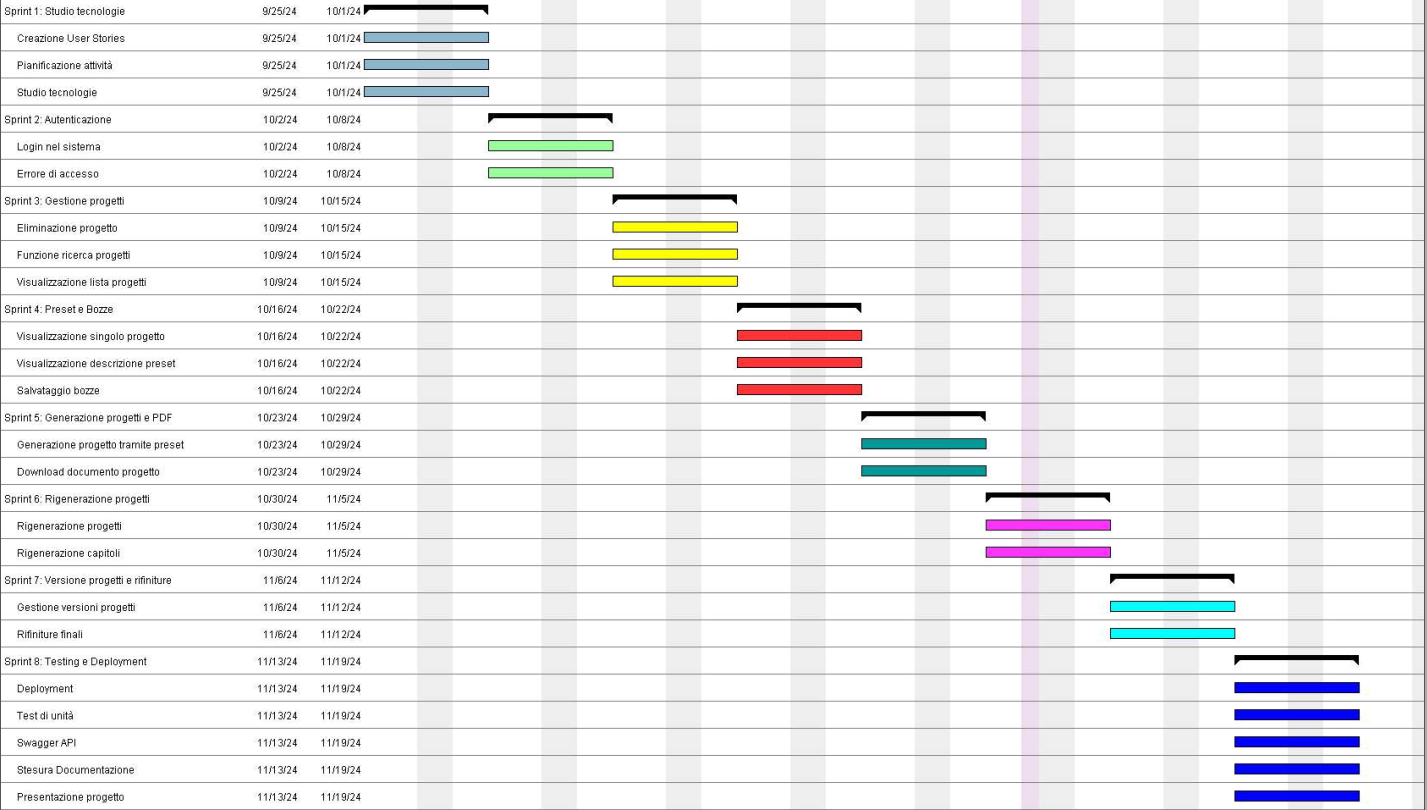
\includegraphics[scale=0.43]{pianificazione/gantt-chart.png}
    \caption{Diagramma di \textit{Gantt} delle attività svolte durante il periodo di stage}
    \label{fig:gantt-chart}
\end{figure}